\ifx\wholebook\relax\else
\input{../Common.tex}
\input{../macroes.tex}
\begin{document}
\fi


\chapter{Parameters and Arguments}\label{ch:argumenting}

\begin{chapterfigure}

\includegraphics[width=0.9\linewidth]{ArgumentTitle}
\end{chapterfigure}

In many previous scripts you sent messages with \emph{arguments}. For example in the message \ct{go: 100} you specified that a robot should move a distance of 100 pixels,  and 100 is the argument of this message. You learned how to define methods but not how to define methods that require arguments. 

In this Chapter, you will learn how to define methods whose behavior can be parameterized, that is whose behavior depends on message argument values. Method parameters act as holes in the method definitions, holes that are filled when the message is sent.  First we will define a method with a parameter and invoke it, then we will analyze it.

%%%%%%%%%%%%%%%%%%%%%%%%%%%%%%%%%%%%%%%%%%%%%%%

\section{Parameter, you say?!}
The method \ct{square} defined in Chapter~\ref{mth:square} is
rather limited because the size of the square is fixed once and for all. You probably asked yourself what should be done to draw a square  300 pixels wide, or 175, or 225 or even 23 pixels wide.  There is nothing preventing you from defining the methods \ct{square300}, \ct{square175}, \ct{square225}, \ct{square23} and so on. 

But if you think about it, creating multiple square methods does not solve the problem we have here. We would rather not define a new method each time. We would like to be able to specify the size of the square without having to define  a new method for every size! For example, we would like to be able to draw squares whose size is given by a user. For that we wouldn't want to define a method.

What we need is a kind of variable whose value will be assigned when the message is sent, and not before. This kind of variable exists in many programming languages and is called a \emph{parameter}. A method parameter is a special variable which can take any value you like \emph{at the moment the message is sent}, not when you defined the method.

Come to think of it, this sounds familiar, doesn't it? After all, you know that methods such as \go or \turnLeft take a value (a distance or an angle) at the time the message is sent. 
Each time you used expressions such as \ct{pica turnLeft: 90}, \ct{pica turnLeft: 32}, or \ct{daly turnLeft: 65}, you defined in the message the value of the angle in the message and the method \ct{turnLeft:} used this value. In fact this was the \emph{same} method \ct{turnLeft:} that was executed with a \emph{different value} as value for the angle to turn. So as you see this is really powerful. Now all you have to do is to understand how to define a method able to take arguments at execution time, like the method \turnLeft can. 


%Method~\ref{mth:gogi}
%\begin{method}\label{mth:gogi}
%go: \textbf{distance}
%    "make the receiver goes forward from a given distance"
%	
%    self goTo: (self positionIfGo: distance)
%\end{method}

\subsection{The method \ct{square:}} You have seen that, in \st, the name of a method is terminated by a colon (\ct{:}) to indicate that the method requires an argument. So if you want to create a method to draw a square with an arbitrary size, we will use \ct{square:} as its name. You define the method \ct{square:} as shown in \methodref{mth:squareArguments}. This method is then used in \scriptref{scr:usesquare}.

\begin{method}\label{mth:squareArguments}
square: \textbf{\emph{size}}
   "Draw a square of the given size"

   4 timesRepeat: 
                    [ self go: \textbf{\emph{size}}.
                    self turnLeft: 90 ]
\end{method}

\begin{scriptwithtitle}{Using the method \ct{square:} }\label{scr:usesquare}
| \caro |
\caro := \Turtle new.
\caro square: 10.
\caro go: 300.
\caro square: 20
\end{scriptwithtitle}

Now let's analyze definition of  method \ct{square:} (\mthref{mth:squareArguments}).  To define a method that requires one  argument, you terminate the method name with a colon \ct{:} and follow it with the name of the parameter, which is \ct{size} in~\methodref{mth:squareArguments}. 

The parameter just represents a variable whose value is defined when the message is sent (not when the method is defined). In the script~\ref{scr:usesquare}, during the first message \ct{square:\ 10} \ct{size} will have the value 10. Then during the message \ct{square:\ 20}, \ct{size} will have the value 20.  The argument, however, does not need to be explicitly declared using vertical bars \ct{|} and \ct{|}.
 
In the method~\ref{mth:squareArguments} the name of the parameter is \ct{size}. The name of the parameter should represent what it is used for. Note that we could have named this parameter \ct{length} as in method~\ref{mth:squareArgumentslength}, or \ct{distance} --- as long as we replace all the occurrences of \ct{size} in the method body with \ct{length}. Note that method~\ref{mth:squareArgumentslength} and  method~\ref{mth:squareArguments} give \emph{exactly} the same results.

\begin{method}\label{mth:squareArgumentslength}
square: \textbf{\emph{length}}
   "Draw a square of the given size"

   4 timesRepeat: 
                    [ self go: \textbf{\emph{length}}.
                    self turnLeft: 90 ]
\end{method}


\section{Practicing}
Now this is time to practice a bit. Let's start with a simple exercise.

\begin{exofigwithsizeandtitle}[0.5]{\includegraphics[width=6cm]{ArgHexagon}}{\ct{hexagon:}}
Define the method \ct{hexagon:} that draws a hexagon with sides of the length passed as argument.
\end{exofigwithsizeandtitle}

\begin{exofigwithsizeandtitle}[0.5]{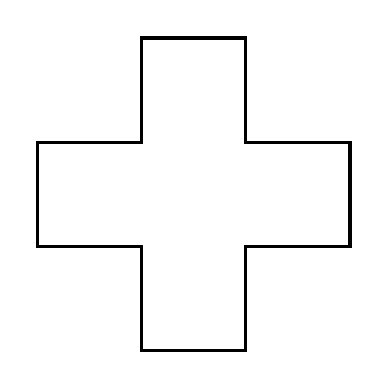
\includegraphics{Argcrossscr}}{Cross}
Transform the script given below into a method named \ct{cross:} that draws a cross of the size that is passed as argument. You should then be able to execute the expression: \ct{\caro\ cross:\ 100}. Hint: notice that 100 / 2 = 50.
\begin{nalltt}
|\caro|
\caro := \Turtle new.
4 timesRepeat: 
               [ \caro go: 50. 
               \caro turnLeft: 90. 
               \caro go: 100. 
               \caro turnRight: 90. 
               \caro go: 100.
               \caro turnRight: 90.
               \caro go: 50 ]

\end{nalltt}
\end{exofigwithsizeandtitle}




%%%%%%%%%%%%%%%%%%%%%%%%%%%%%%%%%%%%%%%%%%%%%%%
\section{Experimenting with Multiple Arguments}
Of course, it would be better to have a method drawing a polygon with a given number of sides \emph{and} size. The question is how do we create a method having two arguments?  You can create a method with two arguments by writing a method name with two colons and placing one argument name after each colon.

\largecadre{To define a method with multiple arguments, terminate each word in the method name with a colon, and place each parameter after its corresponding word in the method name.\\

The method named \ct{polygon:size:} requires two arguments. The definition of the method \ct{polygon: numberOfSides size: size} defines two arguments, \ct{numberOfSides} and \ct{size}.} Its code is shown below. You can then simply send the message \ct{\caro\ polygon:\ 7\ size:\ 100}.




\begin{method}\label{mth:fixedSizePolygon}
\textbf{polygon: numberOfSides size: size}
    "Draws a polygon with the given number of sides and size"

    | angle length |
    angle := 360 / numberOfSides.
    length := 4 * size / numberOfSides.
    sideNumber timesRepeat: 
                               [ self go: length.
                               self turnLeft: angle ]
\end{method}

\paragraph{Implementation Remark.} You may wonder why we defined the length as \ct{4 * size / numberOfSides}. We decided to make the polygon's perimeter equal to the perimeter of a square (\ct{4 * size} is the perimeter of a square. So dividing it by the number of sides and asking a robot to walk that distance the number of sides, makes the robot walking the square perimeter.) that has a side of length \ct{size}. This way the perimeter is constant regardless of the \ct{numberOfSides}, and all the polygons will be displayed using about the same fraction of the screen. 

Here is the code of the method \ct{polygon100:} which draws a polygon with the given number of sides, each side having a length of 100 pixels.

\begin{method}\label{mth:regularPolygon}
\textbf{polygon100: numberOfSides}
    "Draws a polygon with the given number of sides; the length of each
    side is 100 pixels"

    | angle |
    angle := 360 / numberOfSides.
    sideNumber timesRepeat: 
                               [ self go: 100.
                               self turnLeft: angle ]
\end{method}

This method has one argument, \ct{numberOfSides}, and one variable, \ct{angle}. Both of them are used within the code of the method. \ct{numberOfSides}'s value is specified by the message that uses the method, for example \ct{\caro\ polygon100:\ 7}. The variable \ct{angle} is initialized by computing the angle corresponding to the parameter values (namely \ct{360 / 7} in our example). For any value of \ct{numberOfSides}, \ct{angle} will get the right value for the polygon.

\begin{scriptfig}{Arghepta}{Using the method \ct{polygon100:}}\label{src:heptagon}
| \caro |
\caro := \Turtle new.
\caro polygon100: 7.
\end{scriptfig}

You may think that the name of the parameter \ct{numberOfSides} is long. However, this name can easily be understood by any person reading the method. As we already discussed in Chapter~\ref{ch:furthervariables}, it is quite important that anyone be able to read your code --- almost like a story. 

\begin{exonofig}
Define the method \ct{rectangleWidth:height:} which draw a rectangle with the given width and height.
\end{exonofig}

\begin{exonofig}
By slightly modifying the method \ct{cross:}, define the method
\ct{crossWidth:height:} that can draw the crosses shown in
Figure~\ref{fig:c8croix1}.  Note that a normal cross corresponds to
\ct{\caro crossWidth: 30 height: 60}
\end{exonofig}


\begin{figure}[!h]
\begin{minipage}[c]{.3\linewidth}
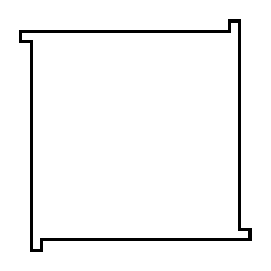
\includegraphics{Argcrossscr2.pdf}
\end{minipage}
\begin{minipage}[c]{.3\linewidth}

\includegraphics{Argcrossscr3}
\end{minipage}
\begin{minipage}[c]{.3\linewidth}

\includegraphics[width=5cm]{Argcrossscr4}
\end{minipage}
\label{c8croix1}
\caption{Three crosses produced by \ct{crossWidth:height:} messages. The cross on the left is from \ct{\caro crossWidth: 5 height: 50}; in the middle, from \ct{\caro crossWidth: 50 height: 5}; on the right, from \ct{\caro crossWidth: 10 height: 20}. \label{fig:c8croix1}}
\end{figure}



%%%%%%%%%%%%%%%%%%%%%%%%%%%%%%%%%%%%%%%%%%%%%%%
\section{Parameters and Variables}
Now that you've practiced a bit, it is time to look  more carefully at the difference between variables and parameters. Let's compare \scriptref{scr:Argsquarewithvariable} and  \methodref{mth:squareArgumentsagain} that I defined earlier (see copies below). 

In \scriptref{scr:Argsquarewithvariable}, first the variable \ct{size} is declared (line 1), then  a value is assigned to it (line 3) and finally it is used as the argument of the method \go (line 5).

\begin{scriptwithtitle}{The square script using a variable}\label{scr:Argsquarewithvariable}
(1)   | \caro \bold{size} | 
(2)   \caro := \Turtle new.
(3)   \bold{size := 10.}
(4)   4 timesRepeat: 
(5)               [ \caro go: \bold{size}.
(6)               \caro turnLeft: 90 ]
\end{scriptwithtitle}

In \mthref{mth:squareArgumentsagain} there are examples of two features of parameters. First, the parameter \ct{size} is declared because it appears after
a colon in the method name (line 1). Second, it is used
as the parameter of the message \go (line 5). A parameter does not have to be initialized because it always gets the value specified in the message that invokes the method. For example when the message \ct{pica square: 20} is sent to \ct{pica}, then the parameter \ct{size} of method~\ref{mth:squareArgumentsagain} gets as value \ct{20}.

\begin{method}\label{mth:squareArgumentsagain}
(1) square: \bold{size}
(2)   "Draw a square of \newcommand{\add}[1]{the} given size"
(3)
(4)   4 timesRepeat: 
(5)                    [ self go: \bold{size}.
(6)                    self turnLeft: 90 ]
\end{method}


\paragraph{No need to declare parameter.}
Unlike other variables, a parameter doesn't have a variable declaration between vertical bars \ct{||}.  A parameter is declared when it appears after a colon \ct{:} in the first line of the method's definition. 

\paragraph{Parameter cannot be assigned.} Another difference is that parameters cannot be modified the way other variables can. You cannot assign new values to parameters inside method bodies. For example, in 
\mthref{mth:squareArgumentsagain} the expression \ct{size := 100} is impossible. 


\paragraph{Variable initialization.} The other difference is the way values are assigned to variables and parameters. A variable value is changed using \ct{:=}.  A parameter value is initialized when the method is executed. For example, \ct{\caro\ square:\ 10} initializes the parameter \ct{size} with the value \ct{10}. A parameter is a variable. However, the  parameter's value is only known when a message is sent and the method executed.

Besides those three differences, a parameter is used in the code of the method like any other variable.




\section{Arguments and Parameters} 
I used the two terms \emph{arguments} and \emph{parameters} for related but different ideas.  An argument is the specific object passed in a message. A parameter is the variable used in a method definition, whose precise value isn't known when the method is defined\footnote{Many authors define these terms differently. Some use "actual parameters" for what we call "arguments", and "formal parameters" for what we call "parameters". Others use the terms "parameter" and "argument" interchangeably.}. 

\begin{figure}[h]
\begin{center}
\includegraphics[width=10cm]{argparam2}
\caption{The connection between an argument (an object) and a parameter (a variable).\label{fig:argparam}}
\end{center}
\end{figure}

In Figure~\ref{fig:argparam}, in the message \ct{square: 100}, the number \ct{100} is the message argument. When the method \ct{square:} is executed its parameter \ct{distance} is initialized to \ct{100}, the value of the argument. 

Another way to understand the difference between an argument and a parameter is that a parameter is a variable inside a method that represents an input  to the method, while an argument is the actual value you pass to this input as shown in Figure~\ref{fig:argparam4}.


\begin{figure}[h]
\begin{center}
\includegraphics[width=8cm]{argparam4}
\caption{The value of the argument is bound to the parameter during the method execution.\label{fig:argparam4}}
\end{center}
\end{figure}


Note that a parameter can also be used as an argument in other message sends. For example in the definition of the method \ct{square:} (method~\ref{mth:squareArguments}), the parameter \ct{size} is used as the argument in the message \ct{go: size}.


A message argument can also be a variable. For example in \scrref{scr:varasArg}, the argument of the first message \ct{square:} is the value of the variable \ct{dist}, that is \ct{100}. The argument of the second message \ct{square:} is the value of the expression \ct{dist + 200}, that is \ct{300}. The parameter \ct{size} of the method \ct{square:} gets the value from the first message, and then the value \ct{300} from the last message. 

\begin{scriptwithtitle}{A variable as argument}\label{scr:varasArg}
| \caro dist |
\caro := \Turtle new.
dist := 100. 
\caro square: dist.
\caro go: 300.
\caro square: dist + 200
\end{scriptwithtitle}








\paragraph{About Method Execution.}
In a first reading you  can simply skip this paragraph since it goes into details that you do not need to know at first. I wrote it because I wanted to answer the questions of the most curious readers but I could have removed this paragraph without problem. When a method is executed new variables are created. These variables are the message receiver, \ct{self}, and the method parameters (that refer to the method arguments) such as \ct{size} in Figure~\ref{fig:argumentswithboxes}. Figure~\ref{fig:argumentswithboxes} shows the effect of sending the message \ct{square: length} to a robot referred to by the variable \ct{pica}, when the variable \ct{length} references the number \ct{100}. 
 
 \begin{figure}[h]
\begin{center}\includegraphics[width=8cm]{argumentBoxes}\end{center}
\caption{When a method is executed, new variables are created that refer to the arguments and the receiver. \label{fig:argumentswithboxes}}
\end{figure}

When the method \ct{square:} is executed, the variable \ct{self} refers to the message receiver, that is the robot pointed to by the variable \caro, and the parameter \ct{size} refers to the value of the variable \ct{length}, that is the number \ct{100}. 
The same process occurs for each message send. For example, the execution of the expression \ct{\daly\ square:\ 200} assigns to \self the robot referenced by the variable \daly, and assigns to \ct{size} the number \ct{200}. 

 
This may look complex but you do not have to worry about it. These are the hidden steps \sq takes to make sure that parameters are initialized with the values in the messages.


\summa

\begin{enumerate}
\item A method parameter is declared right after the colon
  indicating the position of the parameter. It must not be declared as a  variable.
  
 \item To define a method with multiple arguments, terminate each word in the method name with a colon, and place each parameter after its corresponding word in the method name.\\
The method named \ct{polygon:size:} requires two arguments. The definition of the method \ct{polygon: numberOfSides size: size} defines two arguments, \ct{numberOfSides} and \ct{size}.\end{enumerate}


\ifx\wholebook\relax\else\end{document}\fi
